
\documentclass[a4paper, landscape, 6pt]{article}

% --------------------------------------------------------------------------------------------------------------------------------------------------------------------------
\input{./package_and_config.tex}

\def\subject{Mathematik}
\def\semester{2. Semester}
\def\author{Michael Graber, Joshua Kohler, Sven ?, Oliver Schütz}
\def\cols{3}

% Useful packages
\usepackage{amsmath}
\usepackage{graphicx}
\usepackage[colorlinks=true, allcolors=blue]{hyperref}
\usepackage{makecell}
\usepackage{adjustbox}

\title{Mathe 2 Cheatsheet}

\cheatsheet{
    \section{Analysis}
    \subsection{Trigonometrie}
    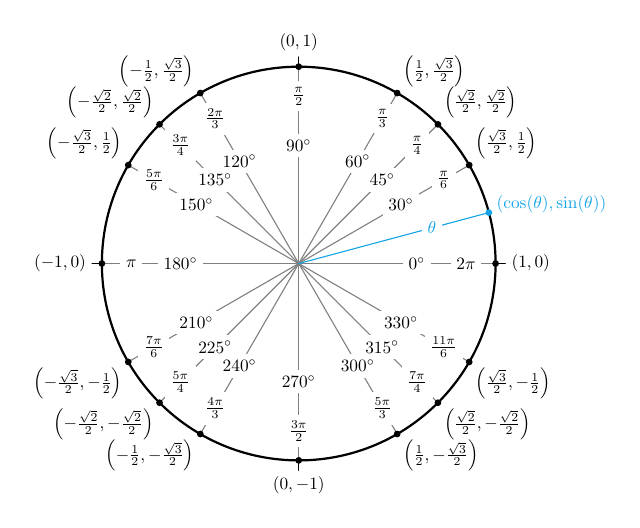
\begin{tikzpicture}[scale=2.5, transform shape, cap=round,>=latex, every node/.style={scale=0.25}] 
    % draw the coordinates
    \draw[-] (-1.05cm,0cm) -- (1.05cm,0cm);
    \draw[-] (0cm,-1.05cm) -- (0cm,1.05cm);

    % draw the unit circle
    \draw[thick] (0cm,0cm) circle(1cm);

    \foreach \x in {0,30,45,60,90,120,135,150,180,210,225,240,270,300,315,330} {
            % lines from center to point
            \draw[gray] (0cm,0cm) -- (\x:1cm);
            % dots at each point
            \filldraw[black] (\x:1cm) circle(0.4pt);
            % draw each angle in degrees
            \draw (\x:0.6cm) node[fill=white] {$\x^\circ$};
    }

    \draw[Cerulean](0cm,0cm) -- (15:1cm);
    \filldraw[Cerulean] (15:1cm) circle(0.4pt);
    \draw (15:0.7cm) node[Cerulean,fill=white] {$\theta$};
    \draw (13:1cm) node[above right,Cerulean] {$\left(\cos(\theta), \sin(\theta)\right)$};

    % draw each angle in radians
    \foreach \x/\xtext in {
        30/\frac{\pi}{6},
        45/\frac{\pi}{4},
        60/\frac{\pi}{3},
        90/\frac{\pi}{2},
        120/\frac{2\pi}{3},
        135/\frac{3\pi}{4},
        150/\frac{5\pi}{6},
        180/\pi,
        210/\frac{7\pi}{6},
        225/\frac{5\pi}{4},
        240/\frac{4\pi}{3},
        270/\frac{3\pi}{2},
        300/\frac{5\pi}{3},
        315/\frac{7\pi}{4},
        330/\frac{11\pi}{6},
        360/2\pi}
            \draw (\x:0.85cm) node[fill=white] {$\xtext$};

    \node[right] at (0:1.05cm) {$\left(1,0\right)$};
    \node[above] at (90:1.05cm) {$\left(0,1\right)$};
    \node[left] at (180:1.05cm) {$\left(-1,0\right)$};
    \node[below] at (270:1.05cm) {$\left(0,-1\right)$};

    \foreach \x/\xtext/\y in {
        150/-\frac{\sqrt{3}}{2}/\frac{1}{2},
        135/-\frac{\sqrt{2}}{2}/\frac{\sqrt{2}}{2},
        120/-\frac{1}{2}/\frac{\sqrt{3}}{2}}
            \draw (\x:1cm) node[above left] {$\left(\xtext,\y\right)$};

    
    \foreach \x/\xtext/\y in {
        30/\frac{\sqrt{3}}{2}/\frac{1}{2},
        45/\frac{\sqrt{2}}{2}/\frac{\sqrt{2}}{2},
        60/\frac{1}{2}/\frac{\sqrt{3}}{2}}
            \draw (\x:1cm) node[above right] {$\left(\xtext,\y\right)$}; 
    
    \foreach \x/\xtext/\y in { 
        210/-\frac{\sqrt{3}}{2}/-\frac{1}{2},
        225/-\frac{\sqrt{2}}{2}/-\frac{\sqrt{2}}{2},
        240/-\frac{1}{2}/-\frac{\sqrt{3}}{2} }
            \draw (\x:1cm) node[below left] {$\left(\xtext,\y\right)$};

    \foreach \x/\xtext/\y in {
        330/\frac{\sqrt{3}}{2}/-\frac{1}{2},
        315/\frac{\sqrt{2}}{2}/-\frac{\sqrt{2}}{2},
        300/\frac{1}{2}/-\frac{\sqrt{3}}{2}}
            \draw (\x:1cm) node[below right] {$\left(\xtext,\y\right)$};
\end{tikzpicture}
    \subsection{Integrale}
    \subsubsection{Substitution}
\textbf{Normale Substitution}\\
\begin{flalign}
    \int_{a}^{b} f(g(x)) dx \quad | \quad u(x) = g(x) \quad &| \quad u'(x) = g'(x) \quad | \quad du = u'(x)\cdot dx \notag&\\
    \int_{u(a)}^{u(b)} u(x) \frac{1}{u'(x)} \,du \quad &| \quad dx = \frac{1}{u'(x)} \,du&\label{eq:Substitution}\\\notag
\end{flalign}
Wenn nach einer Substitution noch ein x in der Gleichung vorhanden ist, muss dieses in ein u umgewandelt werden.

\begin{flalign}
    \int \frac{e^{2x}}{1+e^{2}} \,dx \quad | \quad u = 1 + e^{x} \quad &| \quad u' = e^{x} \quad | \quad du = e^{x} \,dx \Leftrightarrow du = \frac{1}{e^{x}}&\notag\\
    \int \frac{e^{2x}}{u} \cdot \frac{1}{e^{x}} \,du = \int \frac{e^{x}}{u} \,du \quad &| \quad u = 1 + e^{x} \Leftrightarrow e^{x} = u - 1&\notag\\
    \int \frac{u - 1}{u} \,du = \int \frac{u}{u} - \frac{1}{u} \,du &= \int 1 - \frac{1}{u} \,du = \underline{\underline{u - \ln|u| + c}} &\notag
\end{flalign}\\

\textbf{Umgekehrte Substitution (Example)}\\

\begin{flalign}
    \int_{0}^{1} \sqrt{1 - x^2}\, dx \quad &| \quad x = \sin{u} \notag \quad | \quad x' = \cos{u} \notag&\\
    \int_{0}^{\frac{\pi}{2}} \sqrt{1 - \sin^2{u}} \cdot \cos{u}\,du \quad &| \quad dx = \cos{u}\, du \Leftrightarrow   du = \frac{1}{\cos{u}}\, dx \notag&\\
    \int_{0}^{\frac{\pi}{2}} \cos^2{u}\, du \quad =& \quad \left[\frac{u}{2} +  \frac{\sin{2u}}{4}\right]_{0}^{\pi/2} = \frac{\pi}{4} + 0 = \frac{\pi}{4}&\notag
\end{flalign}
    \subsection{Flächen-Integrale}
    \section{Lineare Algebra}
    \subsection{Vektoranalysis}
    \subsubsection{Kreuzprodukt}
\begin{minipage}{\linewidth}
    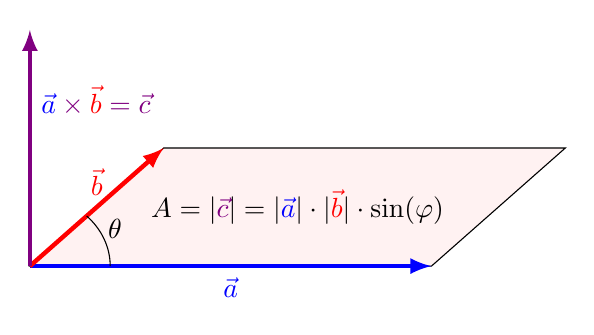
\begin{tikzpicture}[yscale=1.5, xscale=1.7, every node/.style={scale=1}]
    % Rechteck
    \draw[-,fill=white!95!red](0,0)--(3,0)--(4,1)--(1,1)--cycle;
    % Formel in der Fläche
    \node at (2,0.5) {$A = |\textcolor{violet}{\vec{c}} | = |\textcolor{blue}{\vec{a}}| \cdot |\textcolor{red}{\vec{b}}| \cdot \sin(\varphi)$};
    % a
    \draw[ultra thick,-latex,blue](0,0)--(3,0)node[midway,below]{$\vec{a}$};
    % b
    \draw[ultra thick,-latex,red](0,0)--(1,1)node[midway,above]{$\vec{b}$};
    % a x b
    \draw[ultra thick,-latex,blue!50!red](0,0)--(0,2)node[pos=0.7,right]{$\textcolor{blue}{\vec{a}} \times \textcolor{red}{\vec{b}} = \vec{c}$};
    \draw (0.6,0) arc [start angle=0,end angle=45,radius=0.6]
    node[pos=0.7,right]{$\theta$};
    \end{tikzpicture}
\end{minipage}
    \section{Variabletabbele}
    \section{Übungsaufgaben}
}
